% A4 single-column style based on visual_check.tex.
\documentclass[10pt,a4paper,UTF8,fontset=fandol]{ctexart}
\usepackage[margin=1.6cm]{geometry}
\usepackage{graphicx,xcolor,mathtools,amssymb,booktabs,tabularx,multirow}
\usepackage{float,caption,placeins,tikz,needspace}
\usepackage[numbers,sort&compress]{natbib}
\usepackage{xurl}
\usetikzlibrary{arrows.meta,positioning,fit,backgrounds}
\usepackage[colorlinks,linkcolor=blue!55!black,citecolor=blue!55!black,urlcolor=blue!55!black,bookmarksnumbered]{hyperref}
\hypersetup{pdftitle={第一视角人—物交互预测：完整Pipeline技术报告（素材筛选修订版）},pdfauthor={项目技术报告},pdfsubject={手部姿态、物体6D、动态交互图与RSI优化}}
\setlength{\parindent}{0pt}
\setlength{\parskip}{6pt}
\setlength{\intextsep}{12pt}
\renewcommand{\arraystretch}{1.15}
\captionsetup{font=small,labelfont=bf,labelsep=quad,justification=justified,singlelinecheck=false,skip=6pt}
\ctexset{section={format=\Large\bfseries,beforeskip=16pt,afterskip=8pt},subsection={format=\large\bfseries,beforeskip=12pt,afterskip=6pt}}
\setcounter{tocdepth}{1}
\makeatletter
\renewcommand{\l@section}{\@dottedtocline{1}{0em}{2.3em}}
\makeatother
\renewcommand{\refname}{参考文献}
\newcommand{\R}{\mathbb{R}}
\newcommand{\code}[1]{\begingroup\small\ttfamily\def\_{\textunderscore\allowbreak}#1\endgroup}
\pagestyle{plain}
\raggedbottom
\widowpenalty=10000
\clubpenalty=10000
\displaywidowpenalty=10000
\begin{document}
\begin{center}
{\LARGE\bfseries 第一视角人—物交互预测}\\[7pt]
{\Large\bfseries 完整Pipeline技术报告}\\[8pt]
{\normalsize 手部姿态 · 物体6D · 动态交互图 · RSI优化}\\[5pt]
{\small 2026年11月13日\quad 单栏图文版 · 素材筛选修订}
\end{center}

\section*{摘要}

本文介绍第一视角行为意图预测系统的完整技术链：视频与原生时间轴整理、双手21点状态、物体六自由度及表面运动、坐标对齐与监督构建、动态交互图预测，以及基于验证反馈的RSI优化。感知模块分别支持MediaPipe与FoundationPose的RGB-D实测分支，以及官方手姿态与双目重建的EgoDemo数据分支；图预测采用120／132维实体特征、帧内注意力和可替换的Mamba、LSTM、因果Transformer。报告纳入可公开的真人手物、多物体6D与点云演示，新增同一真人视频上从RGB、手部与6D到实际LSTM关系输出的连续演示，并从保存的逐帧数组和日志绘制覆盖、几何一致性与性能验证图。服务器已回收的扩展阶段test micro-F1为LSTM／Transformer 0.938853、Mamba 0.905200；项目方确认最终全量结果约0.93。后续rsi\_final实际账本含30条记录、21个已评分候选，本文给出可复算逐轮曲线，并将其验证成绩与独立测试结果分开。所有图表保留数据版本、输入条件和来源，覆盖从感知到预测的模块原理与实测证据。本版不包含EgoDemo原始画面、记录标识或逐条数据；相关图明确使用原理示意。
\vspace{.2cm}
{\small\tableofcontents}
\clearpage

\section{研究目标与系统概览}
操作行为的提前预测不仅需要知道“发生了什么动作”，还需要判断接下来由哪只手、作用于哪个物体、形成何种关系。手部接近物体可能对应拿取、稳定或即将释放；工具与工件的交互还涉及两个不同客体。单一视频类别难以表达这些结构关系。本项目将可观察的未来交互关系作为行为意图的操作性目标，以有向图统一表达主体、客体与多种并存的关系。

完整系统包括五个环节：视频与原生时间轴整理；手部及物体状态提取；视觉复核与图监督构建；实体编码和时间预测；以及基于验证反馈的RSI优化。系统已经历从小子集联调、自动复核、多采集冻结训练，到位姿增强和后续RSI搜索的连续演进。早期五段实验仅是开发过程中的一个节点，不能替代最终全量结果。

本文重点描述可实现的模块接口和演进关系，而不将收益简单归因于某一个网络。骨干、数据覆盖、监督质量和输入特征在不同阶段均发生变化。评估应先在同一冻结版本内比较，再讨论不同版本之间的工程发展。

\begin{figure}[H]
\centering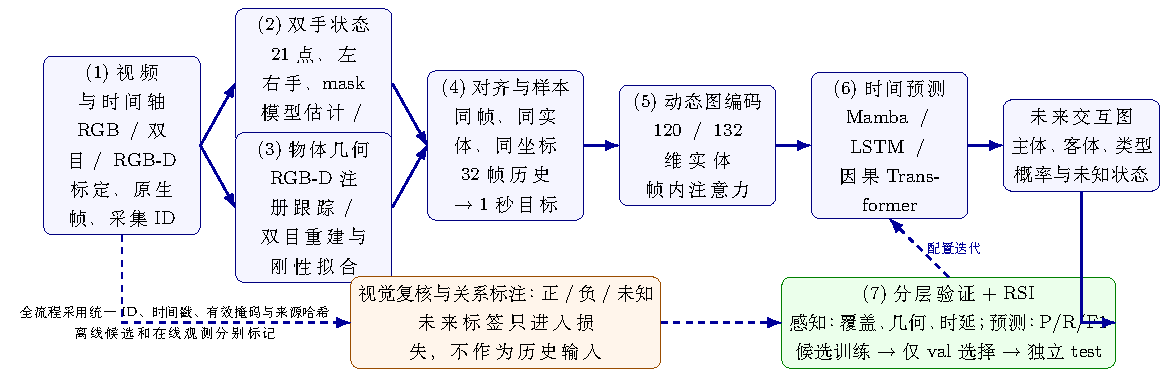
\includegraphics[width=\textwidth]{../04_图片与图表/full_pipeline.pdf}
\caption{完整pipeline与数据流。(2)手部和(3)物体分支并行，(4)统一时间、身份与坐标，(5)(6)学习历史到未来的交互变化，(7)分别验证感知与预测，并驱动RSI配置迭代。未来标签经监督分支进入损失与评估，不进入历史特征；各分支的来源、有效mask和版本随数据传递。}
\label{fig:fullpipeline}
\end{figure}

\paragraph{报告范围。}
本次直接读取了服务器训练配置、评估文件与三个RSI系列账本，并检查本地既有感知输出。项目方确认的最终全量约0.93与已保存的阶段评估分别标明来源；当前rsi\_final目录的验证结果不自动当作独立测试成绩。感知演示与预测测试采用不同数据条件时分别说明，避免把模块通过率拼接成端到端精度。

\section{相关工作}
第一视角数据集EPIC-KITCHENS-100覆盖活动识别、检测与提前预测等任务\cite{damen2022rescaling}；Ego4D拓展了第一视角活动的数据范围\cite{grauman2022ego4d}。本文使用EgoDemo及其本地派生版本\cite{egodemo}，预测具有显式实体引用的未来交互图，不将不同数据集和评价协议的数值直接排名。

手部状态可通过MediaPipe Hands等方法从图像估计\cite{zhang2020mediapipe}，物体六自由度位姿与跟踪可参考FoundationPose\cite{wen2024foundationpose}。项目既有独立RGB-D感知演示，也有使用官方手姿态、审核二维观测和派生几何的训练线路。二者属于不同输入条件；模块演示的帧率不直接等于交互预测全系统的帧率。

Mamba采用输入依赖的选择性状态空间机制，具有沿序列长度线性扩展的特性\cite{gu2023mamba}。本项目将其用作可替换的时间骨干，保留LSTM和因果Transformer作为对照。核心工程设计是统一实体与交互表示、部分监督学习和可回溯的自动优化流程，而非重新提出基础状态空间算子。

\section{原始视频、时间轴与输入条件}
\label{sec:input}
完整pipeline首先确定每个观测对应哪个采集、相机、帧和物理坐标，再进入手部与物体分支。视频切分阶段输出短片及索引，记录来源视频、起止时间、实际帧数与帧率。需要精确边界时重新编码，避免仅按压缩流关键帧切割引入偏移。多相机和同一长视频的不同切片按采集ID分组，训练／验证／测试划分在滑窗之前固定。

第一视角主线保留标注版视频的原生时间戳与相机参数。Raw版与标注版并不保证同一帧号对应同一时刻，必须通过实际长度与时间轴核对。图预测使用32帧历史和至少1秒的未来目标；这与制作视频时使用3fps或10fps回放是不同概念。

系统保留两种可追溯的感知输入条件：EgoDemo线路使用官方手姿态、同采集双目和派生物体几何；独立RGB-D验证线路使用MediaPipe与FoundationPose真实推理。后者用于验证感知模块能运行、可输出什么以及耗时多少，不能直接替代前者的预测测试结果。输入无深度、无尺度或无物体模型时，也不能把另一个RGB-D场景的假设自动转移过去。

\section{手部姿态估计与坐标对齐}
\label{sec:hands}
\subsection{从图像到双手21点}
在线分支采用MediaPipe Hands的两阶段设计：先定位手掌区域，再回归手部关键点\cite{zhang2020mediapipe}。项目封装按帧返回左右手各21点和有效性信息，保留腕部、四指关节与拇指拓扑。未检测到的整只手与置信字段保持NaN，由下游mask明确排除。对非镜像输入按后端自拍约定交换左右手标签；不通过水平翻转原图来掩盖身份错误。

图像输出$(x,y,z_{rel})$中的$x,y$按图像尺寸归一化，$z_{rel}$是腕部相对深度，并非米制相机坐标。左右手分类分数也不是关节定位精度。实时分支和训练数据分支都保留这些语义，避免下游将两个不同坐标空间的量直接相减。

\begin{figure}[H]
\centering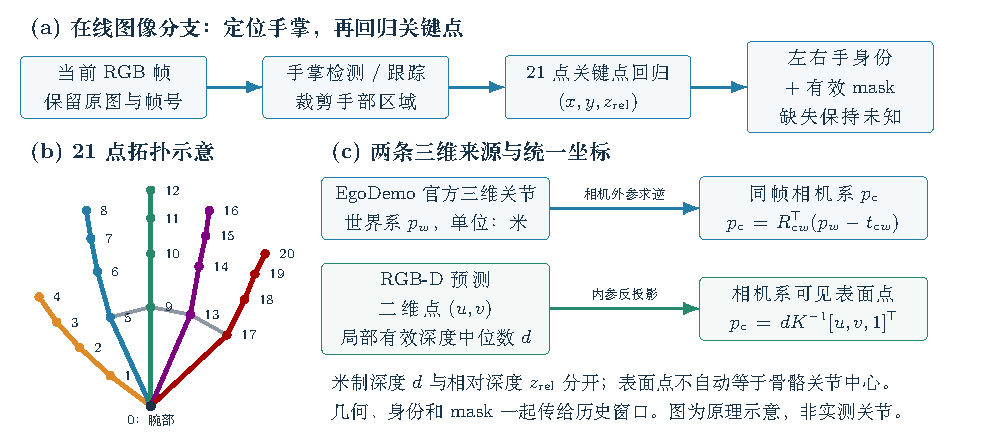
\includegraphics[width=\textwidth]{../04_图片与图表/hand_pose_principle.pdf}
\caption{手部姿态原理图。上：手掌定位到21点回归的在线分支。左下：腕部与五指的21点拓扑。右下：官方世界系关节经相机外参转换，以及RGB-D二维关键点经深度反投影，两条来源分开表达。所有点与模块均为原理示意；坐标图解见图\ref{fig:handcoords}，真实演示见图\ref{fig:rgbdhuman}。}
\label{fig:handprinciple}
\end{figure}

\subsection{官方三维姿态与RGB-D表面提升}
EgoDemo线路读取官方世界坐标手关节和同帧相机到世界变换。若$T_{cw}=[R_{cw},t_{cw}]$表示相机到世界，则
\begin{equation}
 p_c=R_{cw}^{\mathsf T}(p_w-t_{cw}),\qquad
 u=\pi(Kp_c).
\end{equation}
针孔投影$\pi$将齐次坐标除以正深度；负深度、图外点、缺失关节分别保留标记。后续时序特征还会将历史关节转换到锚点相机系，降低头部运动造成的坐标变化。图\ref{fig:handcoords}给出公开版的坐标变换示意。

\begin{figure}[H]
\centering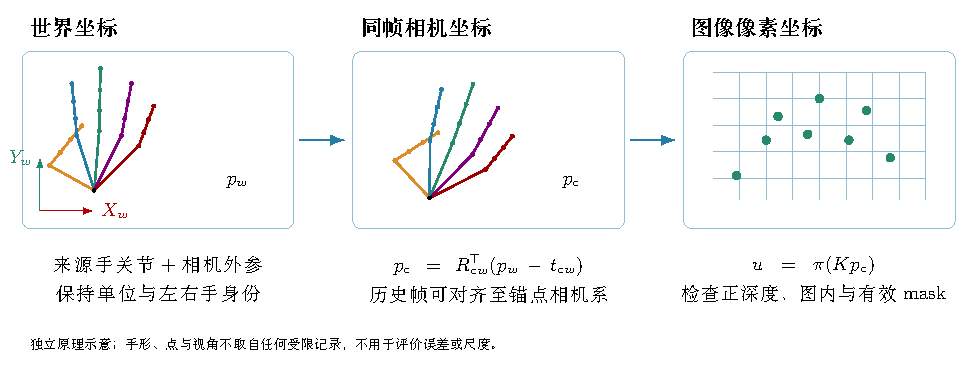
\includegraphics[width=\linewidth]{../04_图片与图表/public_hand_coordinates.pdf}
\caption{手部坐标对齐原理示意。世界系关节由同帧相机外参转换到相机系，再投影到图像；历史关节可进一步对齐到锚点相机系。此图独立绘制，不含EgoDemo原始画面或记录级坐标。真实公开手物例图见图\ref{fig:rgbdhuman}。}
\label{fig:handcoords}
\end{figure}

对有对齐深度的RGB-D输入，可在预测二维关键点附近取有效深度中位数$d$，反投影为
\begin{equation}
 p_c=dK^{-1}[u,v,1]^{\mathsf T}.
\end{equation}
HO-Cap实现使用半径2像素邻域，至少3个有效深度，并限制10\%--90\%分位跨度不超过0.04米。遮挡边缘深度混杂时拒绝提升。这个点表示二维关节射线对应的可见表面，不能自动视为真实骨骼关节的三维中心。

\subsection{真实同帧手物演示}
图\ref{fig:rgbdhuman}左侧展示DexYCB真人持碗的手部预测与物体位姿同时输出；右侧展示HO-Cap四个物体的独立位姿跟踪。它们验证真实模块之间的输入输出衔接，分别保留各自场景和输入条件。工程实现可将手部CPU推理与物体GPU推理并行执行，按同一帧号等待结果齐全后再渲染。

\begin{figure}[H]
\centering
\begin{minipage}{.48\textwidth}\centering
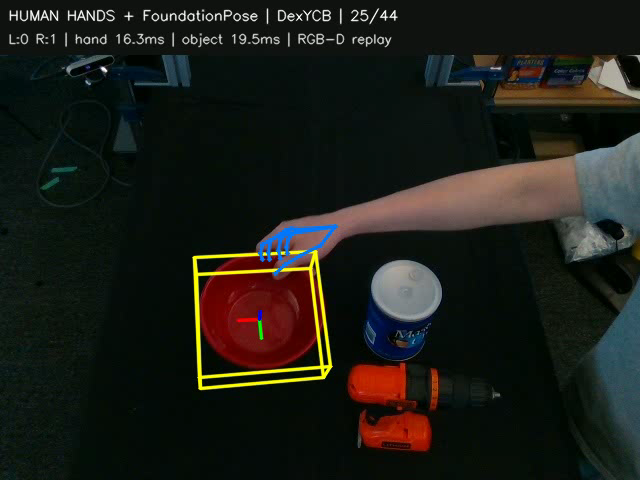
\includegraphics[width=\linewidth]{../04_图片与图表/hand_object_rgbd.png}\\\small (a) DexYCB：21点手骨架、物体框和XYZ轴
\end{minipage}\hfill
\begin{minipage}{.48\textwidth}\centering
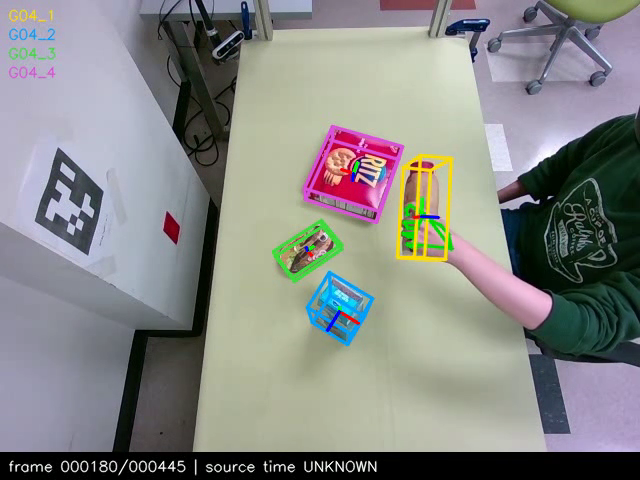
\includegraphics[width=\linewidth]{../04_图片与图表/hocap_four_objects_f180.png}\\\small (b) HO-Cap：同一人手场景中的四物体6D
\end{minipage}
\caption{两条真实RGB-D感知演示，均为既有输出。左图蓝色手骨架来自模型预测；右图从446帧完整视频的第180帧直接解码。颜色区分物体身份，坐标轴表示估计姿态。不同场景不拼接成一次运行；同帧叠加不自动证明手关节与物体已完成独立米制精度验收。}
\label{fig:rgbdhuman}
\end{figure}

\section{物体6D位姿与表面运动建模}
\label{sec:pose6d}
\subsection{六自由度与刚体变换}
6D位姿由平移三自由度和旋转三自由度组成。用物体到相机的齐次变换表示为
\begin{equation}
 T_{oc}=\begin{bmatrix}R&t\\0&1\end{bmatrix},\quad
 R^{\mathsf T}R=I,\quad\det R=1,
\end{equation}
物体模型点$x_o$经$x_c=Rx_o+t$变换后投影到图像。相机运动存在时，用$T_{ow}=T_{cw}T_{oc}$统一到世界系。后续特征中使用旋转矩阵前两列的六维编码；“旋转六维编码”和“物体六自由度位姿”是两个不同概念。

\subsection{RGB-D、mesh与FoundationPose分支}
已知几何模型的RGB-D分支采用FoundationPose\cite{wen2024foundationpose}。注册时输入当前RGB、米制深度、相机内参、目标mask和对应mesh；从姿态候选出发进行学习式细化与评分，随后使用前帧状态和当前RGB-D连续跟踪。项目使用真实scorer／refiner权重，保留原始mesh坐标和返回的物体到相机变换。初始mask与物体匹配，后续跟踪不读取未来位姿参考。

该分支的关键工程约束是单位与物体身份：uint16毫米深度乘0.001后与mesh统一为米；网格不能任意换模型、改尺度或重心而不记录变换。碗等对称物体的朝向可能存在等价解，单看框贴合不能证明全部旋转角精确。图\ref{fig:posecloud}展示预测mesh、估计坐标轴与真实深度点云处于同一相机系的具体输出。

\begin{figure}[H]
\centering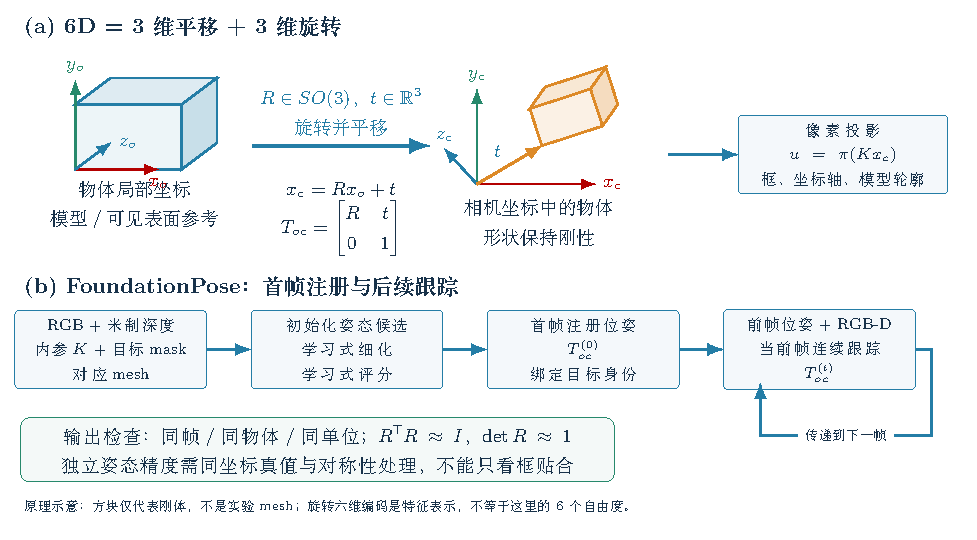
\includegraphics[width=\textwidth]{../04_图片与图表/pose6d_principle.pdf}
\caption{物体6D与FoundationPose原理图。上：物体点由旋转$R$和平移$t$变换到相机系，经内参投影为框、轴或轮廓。下：首帧RGB-D、mask与mesh用于姿态候选细化和评分，后续由前帧位姿与当前观测连续跟踪。图中方块是几何示意，不是实测模型；真实点云与mesh输出见图\ref{fig:posecloud}。}
\label{fig:poseprinciple}
\end{figure}

\begin{figure}[H]
\centering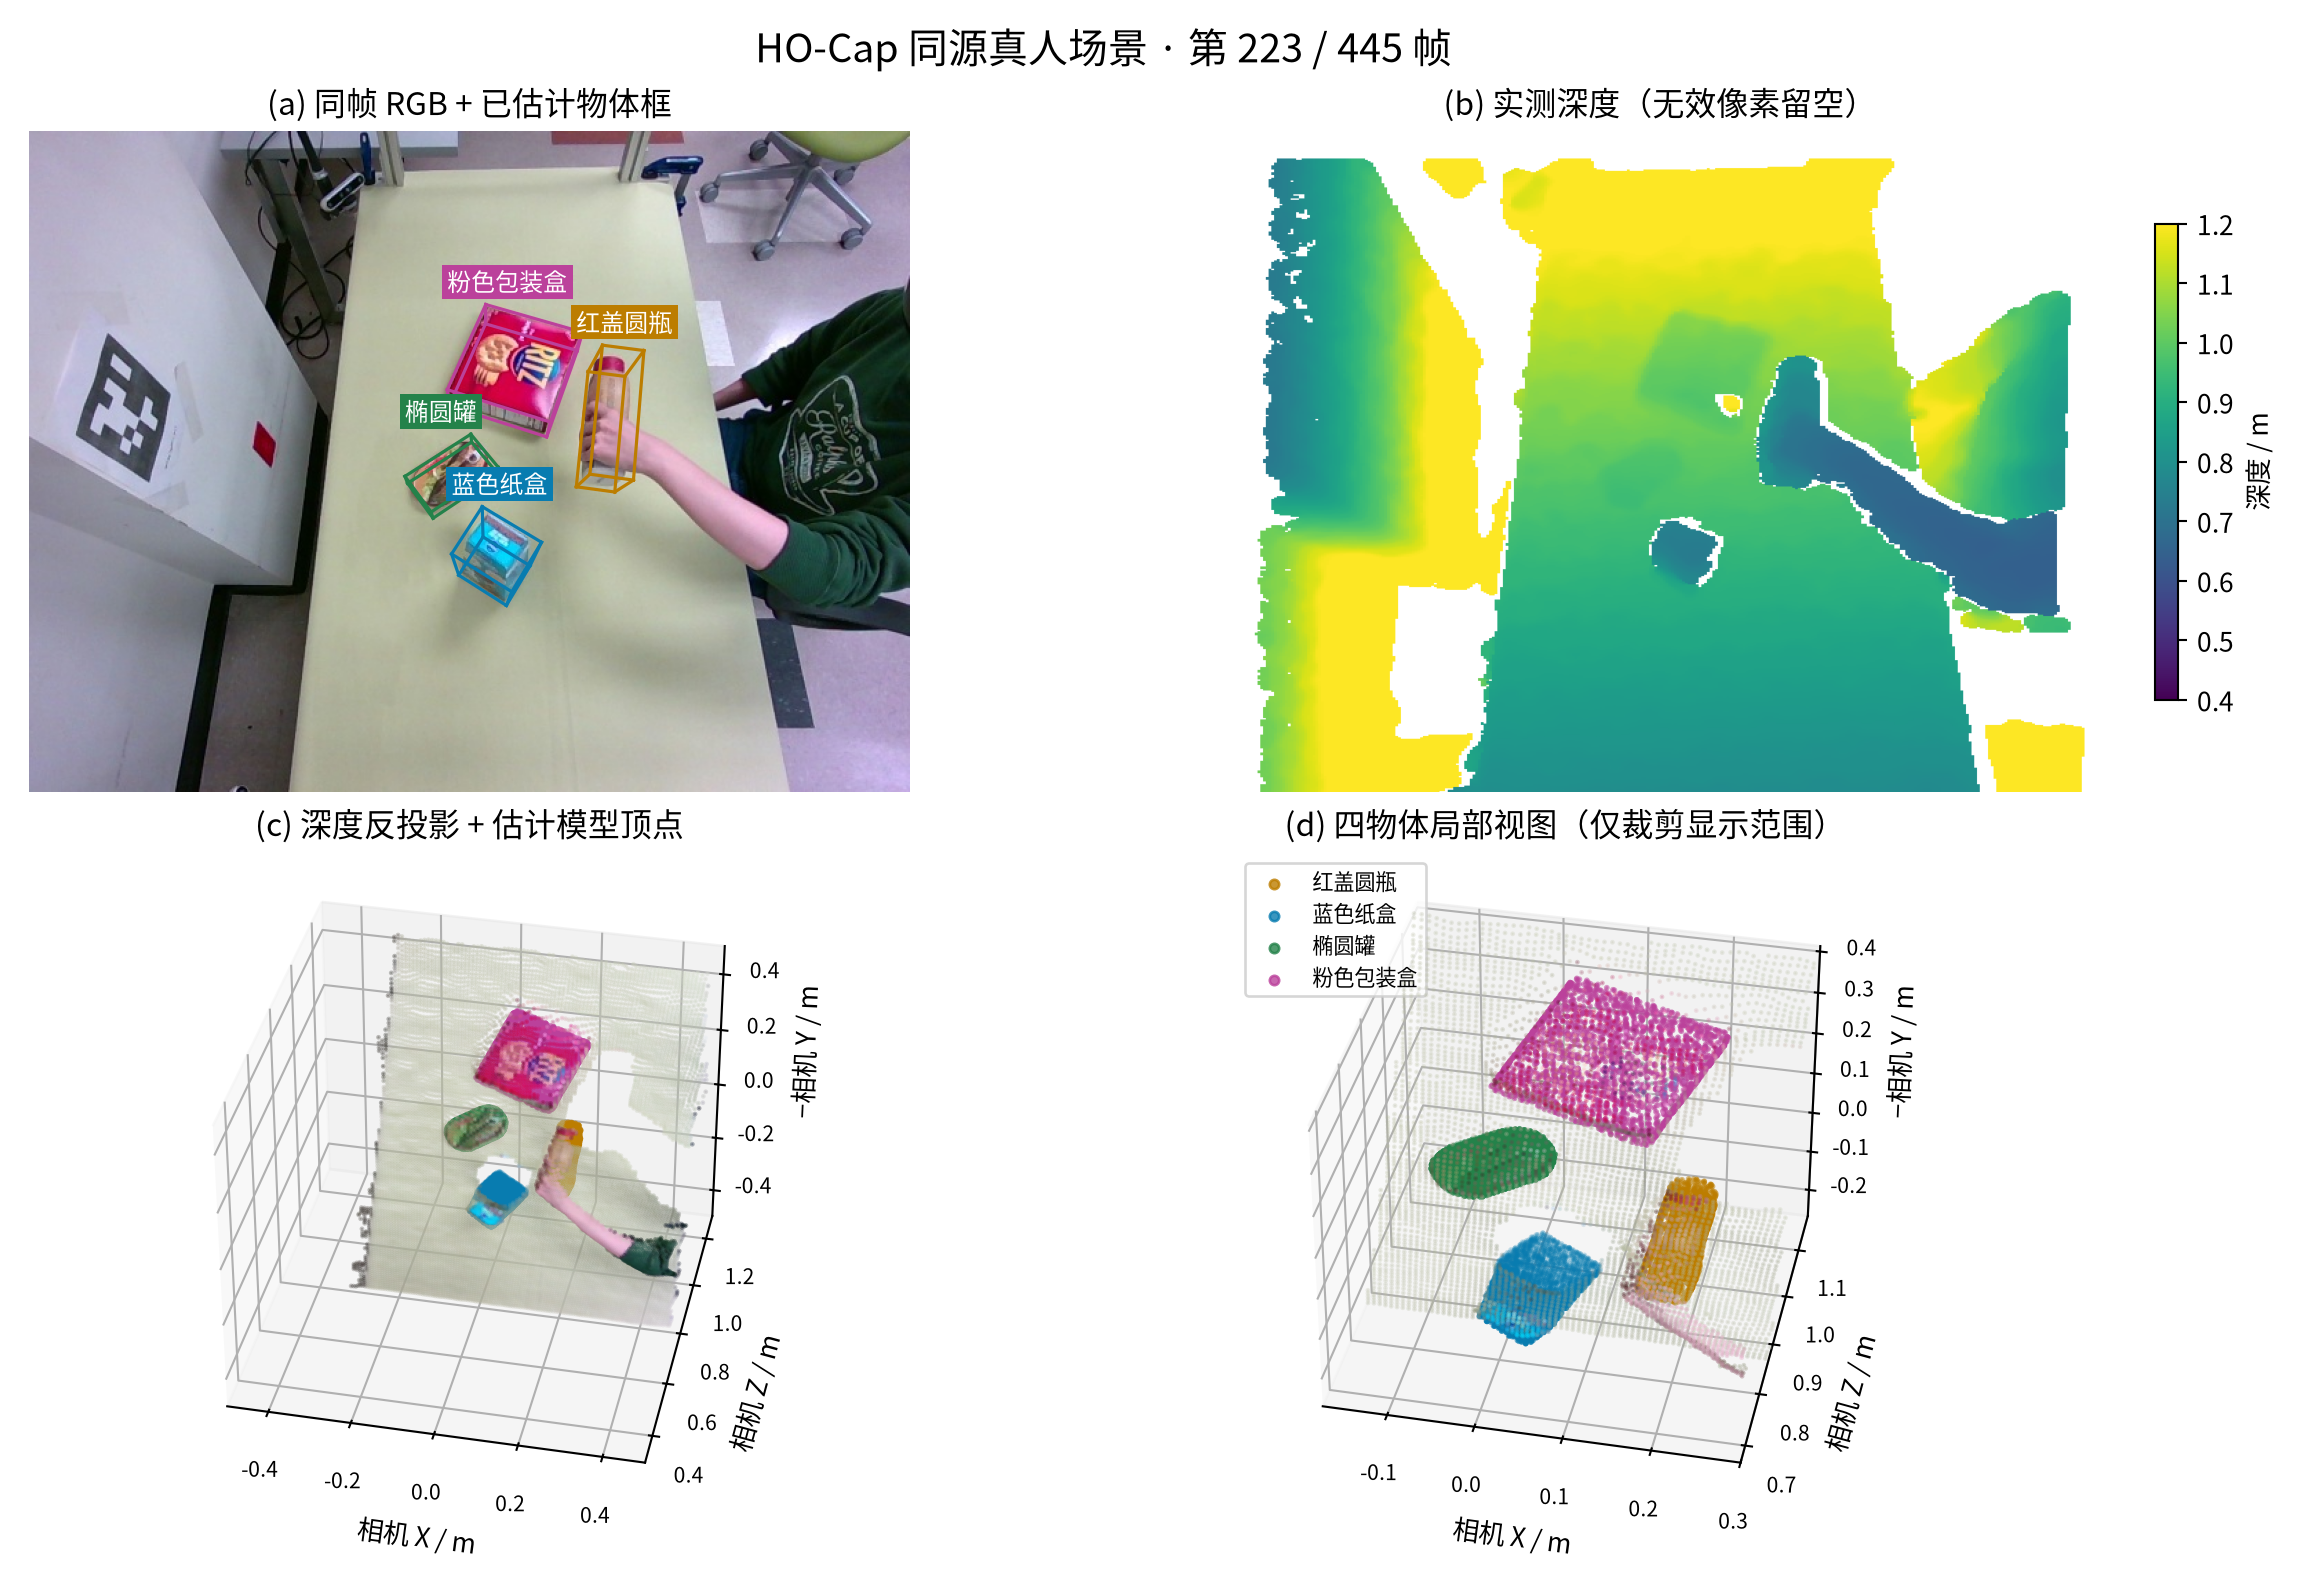
\includegraphics[width=\textwidth]{../04_图片与图表/hocap_same_scene_pointcloud.png}
\caption{与完整流程Demo同源的HO-Cap第223帧：原始RGB、实测深度、反投影点云和估计物体模型。点云由该帧深度及相机内参计算；模型顶点仅应用已保存的FoundationPose位姿，没有利用真值重新对齐。三维视图采用横轴相机X、纵轴相机Z、竖轴负相机Y，单位为米。图示说明坐标对应，不作为独立姿态精度评测。}
\label{fig:posecloud}
\end{figure}

\subsection{EgoDemo双目重建与无CAD几何分支}
第一视角物体通常没有逐个可用的CAD模型，实际工程使用同采集双目、实例表面种子和跨帧点对应来构建局部参考系。相机相对变换为$T_{lr}=T_{rw}^{-1}T_{lw}$。先检查标定与像素对应的一致性，再校正双目、估计视差并进行左右一致性筛选；校正后的理想情形满足$Z=f_xb/d$，非校正情形用双投影矩阵三角化。来源中存在标定修正与留出像素检查，修正记录与原参数同时保留。

连续轨迹提供对应点$\{a_j,b_j\}$，刚性估计求解
\begin{equation}
 (R^*,t^*)=\arg\min_{R\in SO(3),t}\sum_{j\in\mathcal I}
 \|Ra_j+t-b_j\|_2^2 .
\end{equation}
实现用RANSAC剔除错误对应，再对中心化协方差做SVD求$R,t$。本地默认要求至少8个内点、内点比例至少0.65、距离阈值0.012米；同时检查点云跨度与第二奇异值，避免近点状／线状目标的旋转不可观。另有稀疏参考点到后续图像的PnP分支，保留重投影残差与内点数。

物体局部原点来自初始可见表面，轴可由初始相机定义，未必等于CAD中心或语义轴。关联相同名字不代表坐标系已经对齐：跨tracklet拼接还需相对刚体变换和表面一致性证据。纸张、布料等非刚体保留点轨迹或局部表面参考系，铰接工具按部件表达；它们不强制拟合为整物体刚体。

\begin{figure}[H]
\centering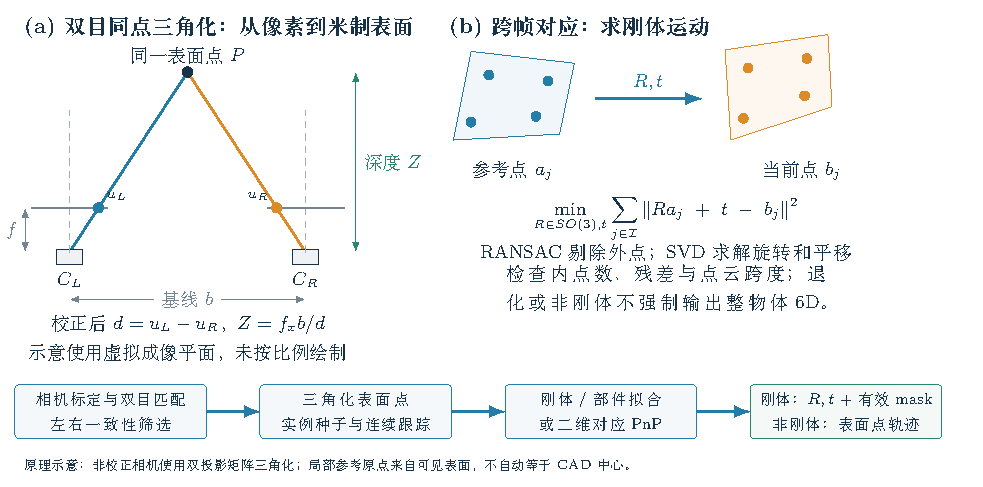
\includegraphics[width=\textwidth]{../04_图片与图表/stereo_geometry_principle.pdf}
\caption{双目重建与跨帧刚体拟合原理图。左上：同一表面点由左右像素射线交会恢复深度，理想校正情形为$Z=f_xb/d$。右上：参考帧与当前帧的对应点，经RANSAC筛选后用SVD求刚体变换。下：从标定、点匹配到局部几何输出的工程路径。相机和点集为原理示意，几何表示区别见图\ref{fig:surface}。}
\label{fig:stereoprinciple}
\end{figure}

\begin{figure}[H]
\centering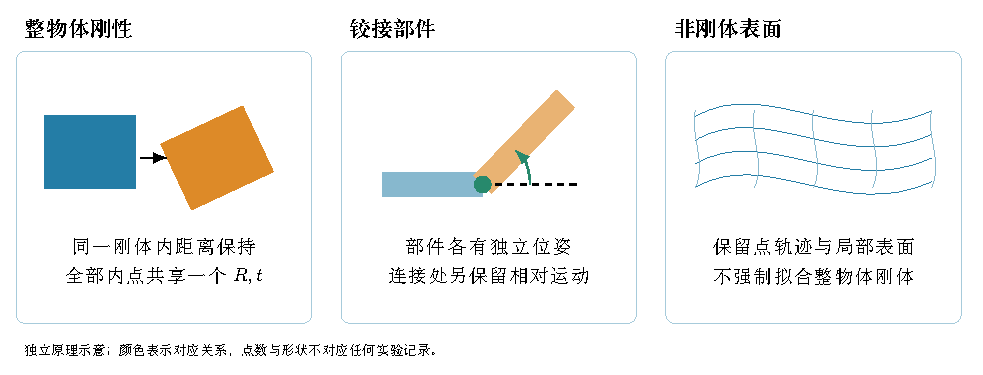
\includegraphics[width=\linewidth]{../04_图片与图表/public_surface_motion.pdf}
\caption{几何表示的三种情况：整物体刚性运动、铰接目标的部件运动和非刚体表面形变。点与形状为原理示意，不是实验数据或受限记录的重建。只有满足刚性约束且对应可靠时，才输出统一物体位姿。}
\label{fig:surface}
\end{figure}

\section{感知模块的指标与验证图}
\label{sec:perceptionmetrics}
\subsection{按指标回答不同问题}
感知验证按输入对齐、输出覆盖、几何一致性、运行时延和独立精度分别报告。覆盖率回答“有多少帧输出有效值”；几何一致性回答“变换、投影与文件是否自洽”；独立精度回答“与外部真值相差多少”。只有具备同物体、同帧、同坐标的独立参考，才能计算位置误差$e_t=\|\hat t-t^*\|_2$及旋转误差
\begin{equation}
 e_R=\arccos\!\left(\operatorname{clip}_{[-1,1]}\!\left(\frac{\operatorname{tr}(\hat RR^{*\mathsf T})-1}{2}\right)\right).
\end{equation}
式中clip限制输入到$[-1,1]$；对称物体需按对称等价类定义评价。手部三维精度可用MPJPE或带阈值的PCK，二维可用独立关键点重投影误差。现有感知材料没有提供完整独立精度评测，因此这些项写为未测，不用覆盖率或轨迹变化替代。

\begin{table}[H]
\centering\small\setlength{\tabcolsep}{5pt}
\resizebox{\textwidth}{!}{\begin{tabular}{llll}
\toprule 环节／验证集 & 已测结果 & 分母与范围 & 结果含义\\\midrule
EgoDemo双手来源检查 & 双手同时有效7146/7164 & 两采集合计7164帧 & 来源姿态覆盖，非检测精度\\
EgoDemo标定像素复核 & 275直接一致，20修正后检查 & 300采集；另4待复核、1不一致 & 抽样像素一致性\\
DexYCB手物联合输出 & 44/44右手与物体均有输出 & 同一44帧，三次复测 & 模块联调与短片覆盖\\
HO-Cap多物体输出 & 446帧；四物体各446有效 & 真人单采集；手任一有效446帧 & 多目标工程覆盖\\
感知独立位置／旋转／手精度 & 未测 & 独立参考尚未形成对应结果 & 不报告虚构准确率\\
\bottomrule
\end{tabular}}
\caption{感知验证结果与统计口径，来自既有运行JSON／NPZ／CSV。不同数据集的计数不相加成为统一测试集。具体失败和缺失状态按各次运行保留，而非覆盖成一个总通过率。}
\label{tab:perception}
\end{table}

\begin{figure}[H]
\centering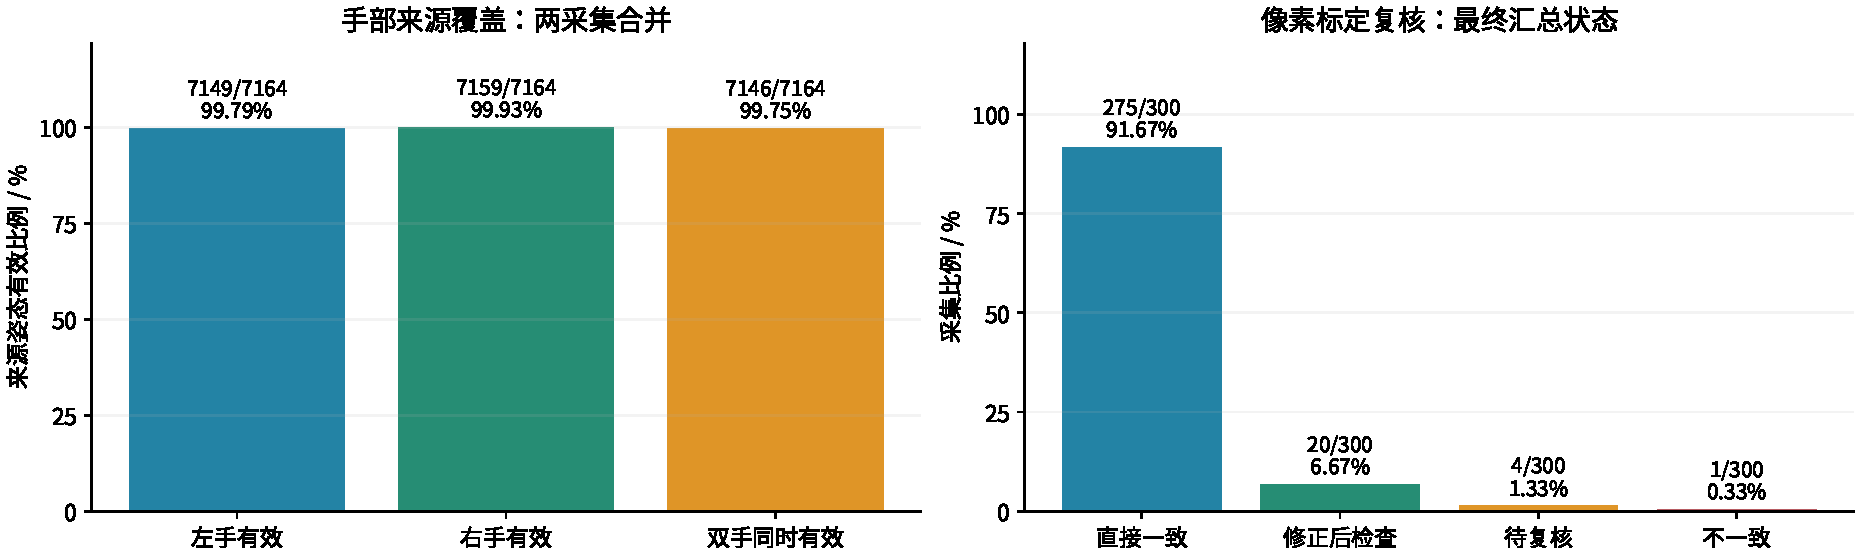
\includegraphics[width=\textwidth]{../04_图片与图表/hand_calibration_coverage.pdf}
\caption{手部来源覆盖与相机像素一致性验证图。左侧为两采集合并的有效帧数与比例；右侧为300段重建流程最终汇总中的标定状态。两者分别验证数据可用性与几何输入，不是学习模型精度。}
\label{fig:coverage}
\end{figure}

\subsection{6D数值验证与逐帧延迟}
图\ref{fig:perceptionvalidation}直接使用当前HO-Cap完整Demo的446帧四物体位姿与手部有效掩码。左图给出四物体与左右手的输出覆盖；中图展示主要操作对象的相机系平移；右图检查四物体旋转矩阵的正交性与行列式。缺失手部观测保留为无效，不补造骨架。平移变化是估计轨迹，矩阵偏差是数值自洽检查，两者都不是与真值比较的误差。

\begin{figure}[H]
\centering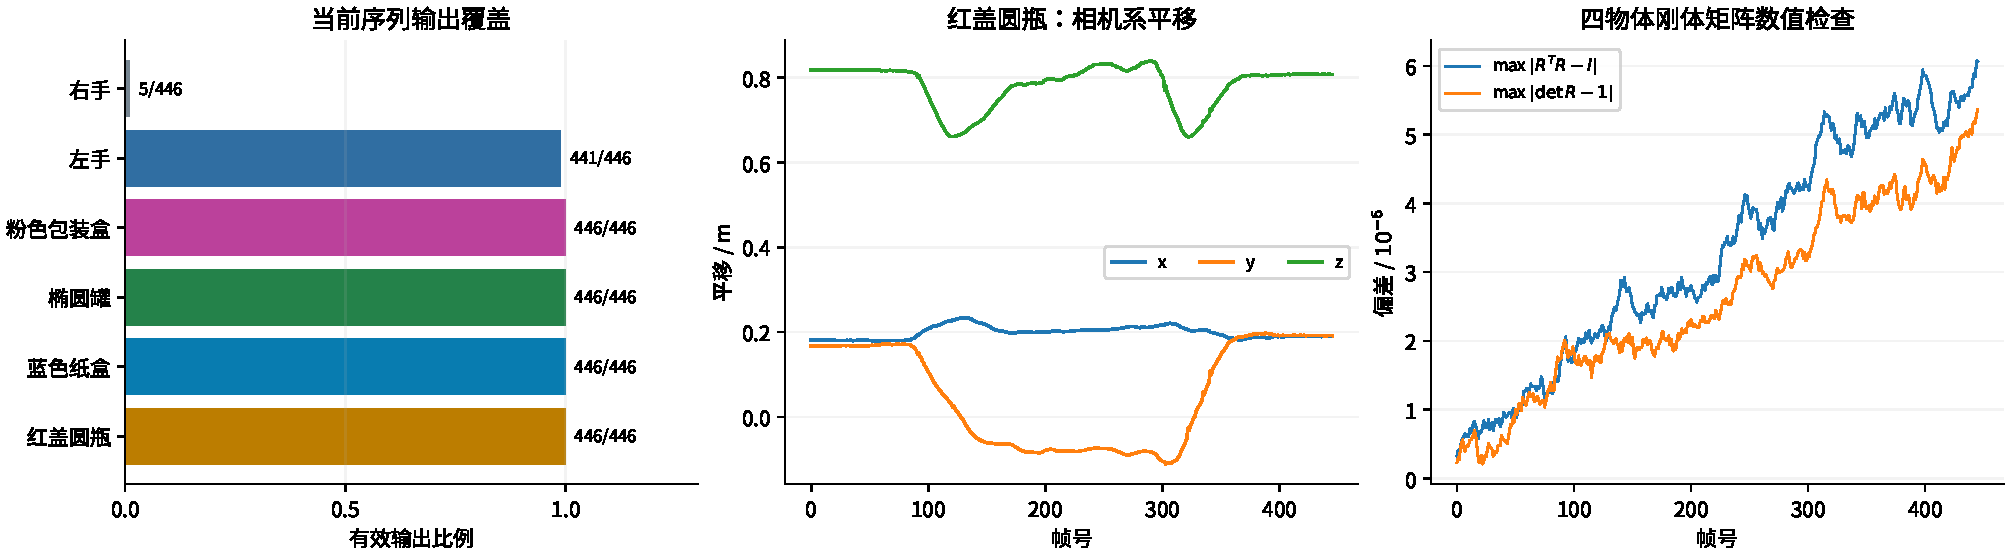
\includegraphics[width=\textwidth]{../04_图片与图表/hocap_perception_validation.pdf}
\caption{当前HO-Cap序列的输出覆盖、红盖圆瓶平移轨迹和四物体旋转矩阵数值检查。覆盖分母为446帧；矩阵曲线每帧取四物体的最大偏差。全部帧参与统计，覆盖与矩阵合法性均不等于独立精度。}
\label{fig:perceptionvalidation}
\end{figure}

\subsection{感知性能优化与实际边界}
同一44帧DexYCB片段在L40上比较不同手模型、物体跟踪迭代和输入预取。最终lite手模型、一次物体跟踪、CPU／GPU同帧并行、有界预取的三次复测稳态处理能力为41.409、41.471、41.524 FPS；帧内P95为27.056、27.967、27.265ms。图\ref{fig:runtime}保留较慢配置，说明优化的实际变化。

\begin{figure}[H]
\centering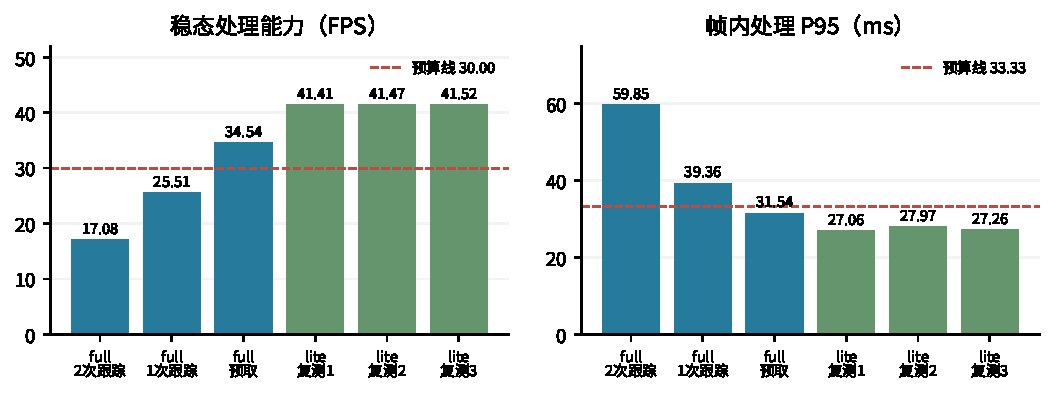
\includegraphics[width=\textwidth]{../04_图片与图表/perception_runtime.pdf}
\caption{真实感知配置的吞吐与帧内P95，均来自同一44帧片段，稳态分母为除注册帧外的43帧。虚线对应30FPS处理预算。改手模型和跟踪迭代数可能影响精度，图中只报告实测性能；三次复测不是132个独立样本。}
\label{fig:runtime}
\end{figure}

最终三轮各有2/43帧超过33.33ms，首帧注册约1.63--1.66秒，读取至写出P95为55.49--66.90ms。因此可以报告短序列稳态处理能力，不能把MP4的30FPS或环路时延写成相机曝光到屏幕显示的硬实时指标。HO-Cap四物体配置的稳态约6.87FPS，单独记录其多物体计算量与输入条件，不套用单碗场景的速度。


\section{数据构建与实验版本}
\subsection{原生时间轴与图监督}
基础资源池包括300段采集、75个原始任务和868,255帧。数据按采集保持原始划分，不把同一采集的不同机位或相邻重叠窗口当作独立视频。采样、审核和训练始终记录采集ID、原生帧号、时间戳、数据版本与来源哈希。

窗口长为32帧，目标帧$u$与历史末帧$t$满足$\tau_u-\tau_t\geq1$秒，实际时间间隔依原生时间戳计算。实体集合包括左手、右手、双手组合和最多八个物体，共$E\leq11$个节点。输出为$E\times E\times66$的有向多标签关系图；66表示冻结词表容量，实际具有监督的类型随发布版本统计。

标签分为操作、关系、转换与协作四层。状态类描述目标帧，转换类表示预测区间内完整包含的已确认事件范围。各单元保存正负值和有效掩码，未检查、遮挡或边界不确定的单元保持未知。未知不是负例，事件范围也不等于精确转换时刻。

\begin{figure}[H]
\centering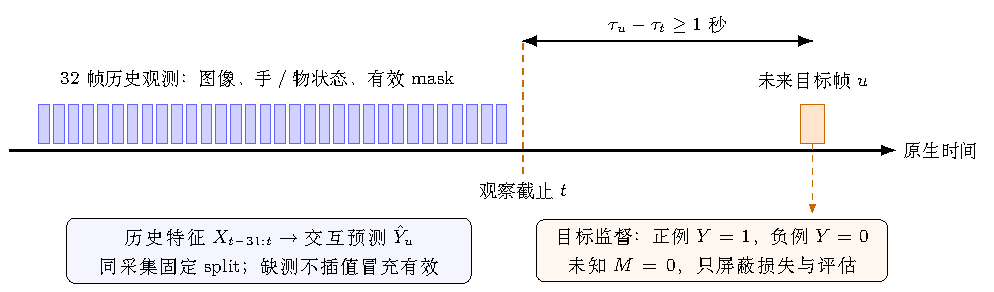
\includegraphics[width=\textwidth]{../04_图片与图表/sample_timeline.pdf}
\caption{时序样本与监督边界示意。历史窗口只使用截止帧及此前的信息，目标由原生时间戳确定；图中方块为结构示意，间隔不表示原视频帧率。正／负／未知分别编码，未来标签不参与输入编码。}
\label{fig:sample}
\end{figure}

\subsection{自动复核与冻结发布}
后续自动化流程包括视觉种子、连续证据渲染、二维跟踪、联系表生成、视觉模型复核与标注组装。复核不仅检查正关系，也单独生成有可见证据的明确负例。接受／拒绝记录保留源图、原生范围、实体引用和判定来源，形成可供加载器验证的发布包。自动视觉复核产生的标签保留银标属性。

发布过程需要在同一冻结点固定索引、数组、标签和证据文件。流水线扩充与训练可以围绕不同版本并行，但冻结过程中继续改写同一证据集合会导致来源不一致。项目迭代曾修复索引导出遗漏、证据配置改变导致像素不一致，以及清理证据文件破坏审计依赖等问题。这些修复的意义在于保证“训练读取的是哪个版本”可被追溯。

\begin{table}[H]
\centering\small\setlength{\tabcolsep}{4pt}
\begin{tabular}{llll}
\toprule 阶段 & 可回溯规模或配置 & 主要变化 & 结果用途\\\midrule
扩展冻结v4（10月26日） & 36/12/9采集；5855/2123/1326窗 & 多采集验证／测试、RSI继续 & 已恢复评估输出\\
后续v7（10月28日） & 42/19/13采集；8049/3329/2757窗 & 继续扩充，V6位姿接入 & 已恢复索引摘要\\
后续fasttrain（11月4日） & 36/7/10有效采集；1012/159/172窗 & 132维、稀疏采样加速 & 独立采样版本\\
最终全量与多轮RSI & 项目方报告最终结果约0.93 & 最终测试文件绑定待确认 & 正式结论的绑定目标\\
\bottomrule
\end{tabular}
\caption{本文涉及的数据版本，斜杠依次为train/val/test。不同数据版本的规模和采样策略不同，不能混为单一试验。fasttrain有效采集数来自本次读取的索引。扩展v4的验证／测试窗口数已与服务器benchmark核对；同名数据根后续曾重新导出，历史运行不直接绑定其当前内容。}
\label{tab:versions}
\end{table}

\subsection{几何增强与覆盖解释}
物体几何由二维观测逐步扩展为刚体／部件位姿、近似刚性集合和非刚体表面参考系。记录中的v10几何扩展使有位姿候选的采集由162段增加到293段，候选位姿帧由274,791增加到699,913。该计数包括不同几何范围，反映候选覆盖，而非全部交互目标的独立6D精度。

后续位姿特征通过视觉实体到几何实体的名称关联接入。早期精确名称匹配漏掉“胶带／黄色胶带卷”等别名，随后加入别名拆分、子串与二元组匹配，提升部分场景的可用性。没有匹配证据的物体仍应保持缺失；非刚体也不能仅因提供一个局部参考系就被称为整物体刚体。
\section{动态交互图预测方法}
\subsection{统一实体特征}
基础版本的每个实体使用 120 维向量：归一化二维框四维、历史速度二维、框内 RGB 均值与标准差六维、手部二维关节 42 维、三维关节 63 维，以及有效性和种子标记三维。物体不具备的手关节字段置零，双手组合节点不伪造独立骨架。无效特征在进入可学习层前通过 $V_t$ 清零，避免 NaN 经线性层污染梯度。三维手姿态统一到历史末帧左相机坐标系，长度单位为米。

节点类别编码仅区分左手、右手、双手与物体四种角色。所有物体共享同一类别嵌入，不加入槽位编号嵌入。基础模型不使用名称嵌入；后续位姿匹配模块会使用中文名称来关联几何，名称关联错误因而可能间接影响输入。目标标签不作为前向特征。

\begin{figure}[H]
\centering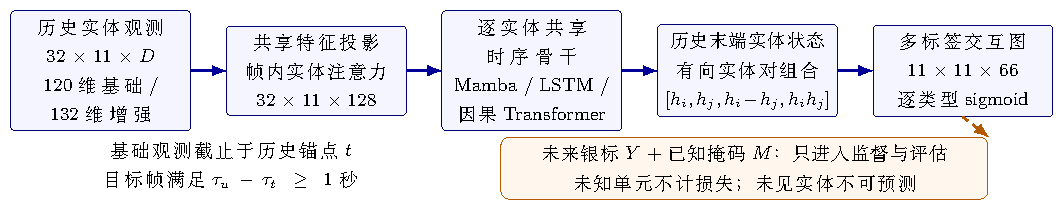
\includegraphics[width=\textwidth]{../04_图片与图表/graph_architecture.pdf}
\caption{系统实现。帧内注意力建模空间上下文，时间骨干沿各实体历史独立且共享地运算；末端有向图头保留主体与客体的区别。同一数据版本内的三骨干对照替换时间模块；132维位姿增强另记录离线来源。虚线表示损失与标签的关联，标签不进入前向特征。图为实现结构示意，不是实验输出。}
\label{fig:architecture}
\end{figure}

\subsection{帧内关系编码}
以基础配置为例，首先用共享两层感知机将实体特征投影至 $d=128$ 维，再加入实体类别嵌入。每帧的所有有效实体共同参与四头注意力：
\begin{align}
 Z_{s,i}&=\phi(X_{s,i})+e_{\kappa(i)},\\
 \widetilde Z_s&=\operatorname{LN}\big[Z_s+
 \operatorname{Attn}(\operatorname{LN}(Z_s);V_s)\big].
\end{align}
无效实体作为 key 被屏蔽，输出也重新置零。若整帧没有有效观测，实现暂时保留一个零值 key 防止全负无穷 softmax 产生 NaN，再屏蔽该帧所有输出。该步骤处理数值稳定性，不把缺失帧变为有效观测。

帧内注意力让手部节点能依赖附近物体的状态，同时使物体表示包含其他实体的上下文。这里的注意力权重不是物理接触标签，模型最终是否识别接触仍需由独立监督检验。

\subsection{共享时间骨干}
将张量由 $B\times W\times E\times d$ 重排为 $(BE)\times W\times d$，基础配置使用共享两层时间骨干建模每个实体的历史；RSI候选的宽度和层数由其配置确定。在 Mamba 分支中，状态维数为 16，局部卷积宽度为 4，扩展倍率为 2。选择性状态更新可抽象写作
\begin{align}
 H_{s,i}&=\overline A_{s,i}H_{s-1,i}
             +\overline B_{s,i}\widetilde Z_{s,i},\\
 O_{s,i}&=C_{s,i}H_{s,i},
\end{align}
其中与输入相关的系数选择保留哪些历史信息；实际计算使用现成的 \code{mamba\_ssm} 实现。此式说明机制，并不省略后声称为完整软件层公式。

LSTM 分支采用相同宽度和层数的循环时间模块。Transformer 分支使用可学习时间位置编码、上三角因果屏蔽和四倍宽度的前馈层。三者共享实体编码器、图头、输入、标签与优化规则，但参数量不保证相等，因此本实验是接口和训练协议对齐的骨干比较，不是等参数量或等算力的严格对照。

历史中曾出现但在后续帧缺失的实体允许保留时间状态；从未出现的实体始终屏蔽。固定物体槽并不等于固定物理身份；只有在历史观察提供对应依据时，该节点才具备可解释的实体引用。

\subsection{有向图解码与损失}
在窗口末端提取实体状态 $h_i$，按有序实体对组合
\begin{equation}
 r_{ij}=[h_i;h_j;h_i-h_j;h_i\odot h_j],
\end{equation}
并通过共享感知机产生 $K$ 个 logits $\ell_{ij}$。顺序拼接和差向量保留方向性，使“手作用于物体”和“物体受到手作用”不会被自动视作同一边。每类独立 sigmoid 适用于多标签关系，不使用互斥 softmax。图头支持手到物体以及物体到物体的组合；下游解释仍须遵守类型语义，不能把任意高分组合都认作物理上有效的交互。

令 $Q_{ij}$ 表示源和目标均在历史中出现。训练仅使用既有标注又满足预测条件的单元：
\begin{equation}
 \mathcal L=\frac{1}{|\Omega|}
 \sum_{(i,j,k)\in\Omega}
 \operatorname{BCEWithLogits}(\ell_{ijk},Y_{ijk}),
\end{equation}
其中 $\Omega=\{(i,j,k):M_{ijk}=1,\ Q_{ij}=1\}$。实现会拒绝指向历史未见实体的监督，而不是悄悄丢弃该项。未知单元不进入损失，FP32 累积 BCE 以降低混合精度误差；空监督 batch 必须显式跳过或报告，不能冒充有效训练。

物体槽位置换只改变节点排列；共享类别编码、帧内集合注意力、共享时间模块和共享实体对头使图预测随槽位相应置换。已有冒烟审计记录的最大绝对差为 $1.788\times10^{-7}$。这证明特定检查下的实现一致性，不等于在任意身份错误下仍能正确预测。


\subsection{132 维位姿增强与实体关联}
后续 V6 将输入扩展为 $120+12=132$ 维。新增块依次为位置三维、旋转六维表示、位姿有效标记、离线候选标记和一维保留位。旋转编码为旋转矩阵的前两列；物体局部位姿经相机到世界变换对齐至世界坐标。无匹配或无效帧的块置零，并由有效标记区分，不用零位置冒充有效物体位置。

\code{PoseTable} 将视觉实体与 v10 几何轨迹关联：先保留并拆分原始名称中的别名，再进行归一化；匹配分数优先考虑名称相等，其次子串关系，最后字符二元组的 Jaccard 重叠。当前代码以 0.34 为最低接受分数。这是工程关联规则，可能把语义接近而物理上不同的实例匹配在一起，故报告和 demo 需保留关联置信与缺失状态。

v10 几何包含整物体、刚性部件、近似刚性集合与非刚体表面参考系。后两者能提供局部运动描述，但不能全部改称整物体刚体 6D。当前位姿块显式带有 \code{offline\_pose\_candidate} 标记，来源可能使用离线信息。因此 120 维历史观测实验与 132 维离线几何增强实验应分别报告；将块附到历史帧上，并不自动证明上游位姿估计本身因果。

\section{RSI自动迭代优化}
\subsection{候选生成与训练}
RSI将一次优化抽象为“当前配置→受约束变异→候选训练→验证评分→候选晋升”。每个候选保存独立目录和配置，避免后续轮次覆盖此前训练结果。现有实现支持切换Mamba、LSTM和Transformer，并在白名单中修改网络宽度、层数、dropout、batch size、学习率、权重衰减及checkpoint选择指标。

\begin{table}[H]
\centering\small
\begin{tabular}{ll}
\toprule 配置项 & 本地RSI实现的搜索集合\\\midrule
隐藏维度 & 64、128、256\\
时间层数 & 1、2、3、4\\
dropout & 0、0.1、0.2\\
batch size & 8、16、32\\
学习率 & $10^{-4}$、$3\times10^{-4}$、$10^{-3}$\\
权重衰减 & 0、0.01、0.1\\
轮内选优 & val loss／micro-F1／macro-seen\\
\bottomrule
\end{tabular}
\caption{搜索空间来自\texttt{rsi\_v5.py}。最终运行的候选集合以实际history与配置为准，不由默认参数推算完成轮数。}
\end{table}

数据路径、输入语义和标签词表不属于这段随机变异的搜索对象。切换数据发布或120／132维特征时应开启有明确版本绑定的新系列，而不是把它解释成同一系列内的一次普通超参变异。RSI可同时使用验证损失选择某个候选内部的checkpoint，再使用验证micro-F1在候选之间比较；这两个选择层次应分别记录。

\subsection{验证选择、失败处理与晋升}
已检查实现的候选评分为验证micro-F1，只有新分数超过当前分数的1.02倍时才晋升；该2\%相对阈值是搜索启发式，不是统计显著性检验。训练退出非零、评估失败或缺少benchmark的候选记录为失败，不以零分或未完成结果冒充成功试验。搜索过程只调用val，胜者的test评估在外部执行。

候选目录、\code{history.jsonl}、\code{score.json}、\code{genome.yaml}与汇总报告共同保存实验谱系。历史有多个系列：\code{rsi\_v5}、\code{rsi\_auto}和后续\code{rsi\_final}。不能将每个系列的默认八轮累加为实际成功轮数，也不能把失败后重跑的同一候选重复计算为新模型。最终需要报告总尝试数、唯一候选数、成功评分数、晋升序列及冠军配置。

\begin{figure}[H]
\centering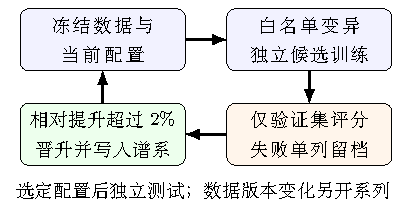
\includegraphics[width=.65\linewidth]{../04_图片与图表/rsi_loop.pdf}
\caption{RSI机制图。该图说明代码流程，不代表已完成轮数或各轮收益。}
\label{fig:rsi}
\end{figure}

\subsection{服务器账本与实际轮次}
本次直接回收三个系列的\code{history.jsonl}、\code{score.json}、配置与benchmark。\code{rsi\_v5}和\code{rsi\_auto}各有8条轮次记录、6个唯一候选；\code{rsi\_final}有30条记录、21个唯一已评分候选，另有一个候选目录尚无score文件。重复出现的候选复用既有评分，因此不能把46条记录称为46个独立模型，也不将当前无score的目录算作成功实验。

\begin{table}[H]
\centering\small\setlength{\tabcolsep}{4pt}
\begin{tabular}{lrrr}
\toprule 系列 & 记录数 & 唯一已评分 & 最高val F1\\\midrule
rsi\_v5 & 8 & 6 & 0.856580\\
rsi\_auto & 8 & 6 & 0.914068\\
rsi\_final & 30 & 21 & 1.000000\\\bottomrule
\end{tabular}
\caption{服务器快照中的RSI账本，三个系列对应不同数据版本。表中最高分不必等于当前genome，是否晋升还受2\%相对阈值约束。}
\label{tab:rsiobserved}
\end{table}

\begin{figure}[H]
\centering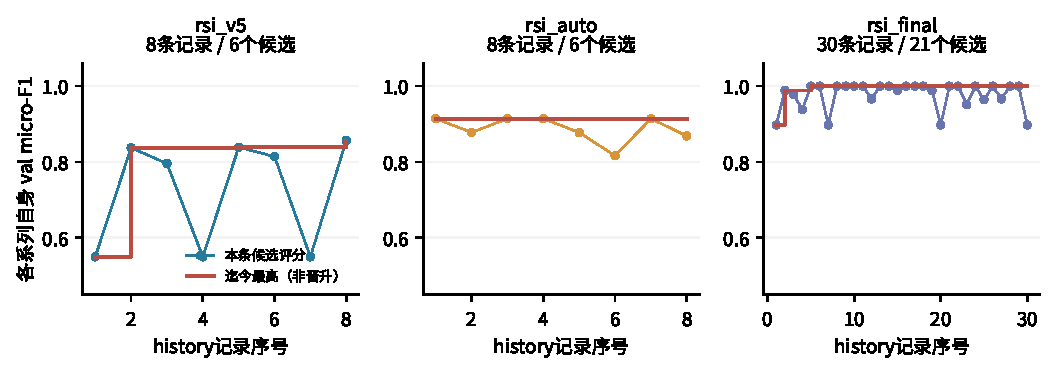
\includegraphics[width=\textwidth]{../04_图片与图表/rsi_observed_history.pdf}
\caption{由三个实际history逐条复算的RSI曲线。横轴为账本记录序号，保留重复候选复用；红线为迄今最高分，不冒充晋升记录。各系列的验证集不同，分面展示而不连接为同一测试集上的提升。}
\label{fig:rsihistory}
\end{figure}

后续\code{rsi\_final}使用132维输入、fasttrain数据、80个epoch上限及验证micro-F1选优。当前genome为两层64维LSTM、batch size 16、学习率$3\times10^{-4}$、权重衰减0.01；其保存的验证F1为0.988506。存在1.0候选，但从0.988506到1.0不足2\%相对提升，不能仅按最高候选值认定genome已经晋升。

这一验证集为159窗口、275个已知单元，含43个接触正例与232个抓持负例。1.0仅表示该监督分布上的验证得分，不表示66种交互均得到验证，更不能替代最终独立测试。当前三个\code{*\_final}目录保存了模型和配置，但未发现对应test benchmark；保留项目方最终约0.93声明，后续应与指定最终运行绑定。

\section{实验结果与版本对应}
\subsection{已恢复的扩展数据评估}
表\ref{tab:results}已直接核对服务器\code{graph\_v5\_auto/*\_auto\_v4/eval/}中的评估JSON；与历史工具输出一致。该输出属于扩展冻结数据阶段，已不再是五段试点。LSTM和Transformer的test micro-F1为0.939，Mamba为0.905；验证F1分别为0.816、0.872和0.807。

\begin{table}[H]
\centering\small\setlength{\tabcolsep}{6pt}
\begin{tabular}{lrrrrrrrr}
\toprule & \multicolumn{3}{c}{验证集} & \multicolumn{5}{c}{测试集}\\
\cmidrule(lr){2-4}\cmidrule(lr){5-9}
模型 & BCE & micro-F1 & Precision & BCE & Precision & Recall & micro-F1 & macro-seen\\\midrule
Mamba & 0.436 & 0.807 & 0.873 & 0.352 & 0.889 & 0.922 & 0.905 & 0.907\\
LSTM & 0.491 & 0.816 & 0.856 & 0.297 & 0.885 & 1.000 & 0.939 & 0.943\\
Transformer & 0.421 & 0.872 & 0.849 & 0.318 & 0.885 & 1.000 & 0.939 & 0.943\\
\bottomrule
\end{tabular}
\caption{扩展冻结阶段的已记录评估值。数值已从服务器评估JSON核对，非本轮重新训练；表格显示三位小数。LSTM／Transformer精确test micro-F1为0.9388532001，Mamba为0.9052002986；测试1326窗口。该阶段采用120维输入，不冒充132维RSI的独立测试。}
\label{tab:results}
\end{table}

\begin{figure}[H]
\centering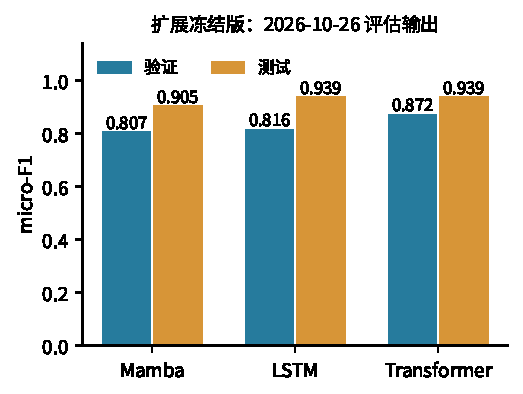
\includegraphics[width=\linewidth]{../04_图片与图表/expanded_results.pdf}
\caption{扩展冻结版本的验证／测试micro-F1。不同骨干处于同一记录阶段；未提供重复运行方差，故不绘制误差条。}
\label{fig:expanded}
\end{figure}

上述成绩支持系统在扩展数据阶段已经达到约0.94的测试F1。LSTM与Transformer的聚合P/R/F1相同，并不意味着它们对每个窗口的预测完全相同；需要逐单元输出才能比较错误分布。Mamba在该阶段的测试F1低3.4个百分点，而RSI的搜索空间包含骨干选择，因此应以最终胜者的实际配置描述交付模型，不能预先假定冠军一定是Mamba。

\subsection{最终全量结果与后续132维实验}
\textbf{项目方确认最终全量结果约为0.93，并经过多轮RSI优化。}本次已直接读取后续训练配置和30条RSI记录，确认132维特征与多轮搜索实际存在。服务器保存的扩展阶段精确测试结果为0.9388532001，包含TP=3946、FP=514、FN=0；这是可直接核验的一项约0.93结果。

与此同时，后续fasttrain发布的有效窗口为1012/159/172，对应有效采集36/7/10；其RSI账本是验证评分，未附最终独立测试文件。本文因此同时保留项目方最终声明、扩展阶段原始测试和后续RSI验证三类记录，不仅凭数值接近、目录名或较高val分数认定它们是同一次实验。最终冠军指定后，应在相应索引和checkpoint下补齐主结果的唯一绑定。

\subsection{评价口径与基线}
不同数据版本的测试采集、监督分布和输入条件不同。RSI收益应比较同一冻结数据、同一特征和同一评估口径下的初始配置与冠军。全正预测的参照值为$F_1^{all+}=2P/(2P+N)$，其中$P,N$为该版本已知监督的正负单元数；应与相同测试集的模型结果一起计算，不能跨版本比较。

\section{完整流程的连续Demo与可视化}
\subsection{同一视频上的真实输出}
2026年11月13日新增连续三栏演示：左栏在HO-Cap原始RGB上标出红盖圆瓶、蓝色纸盒、椭圆罐、粉色包装盒，并显示实物缩略图；中栏为同帧MediaPipe手部与FoundationPose四物体6D，以及视觉复核的当前交互阶段；右栏为现有LSTM权重产生的“主体—关系—客体”候选及概率。446帧全部连续显示；前31帧积累历史，随后415帧有实际推理结果。原始视频、感知结果和模型输出按同一帧号对齐，图\ref{fig:demo}为实际导出帧。

\begin{figure}[H]
\centering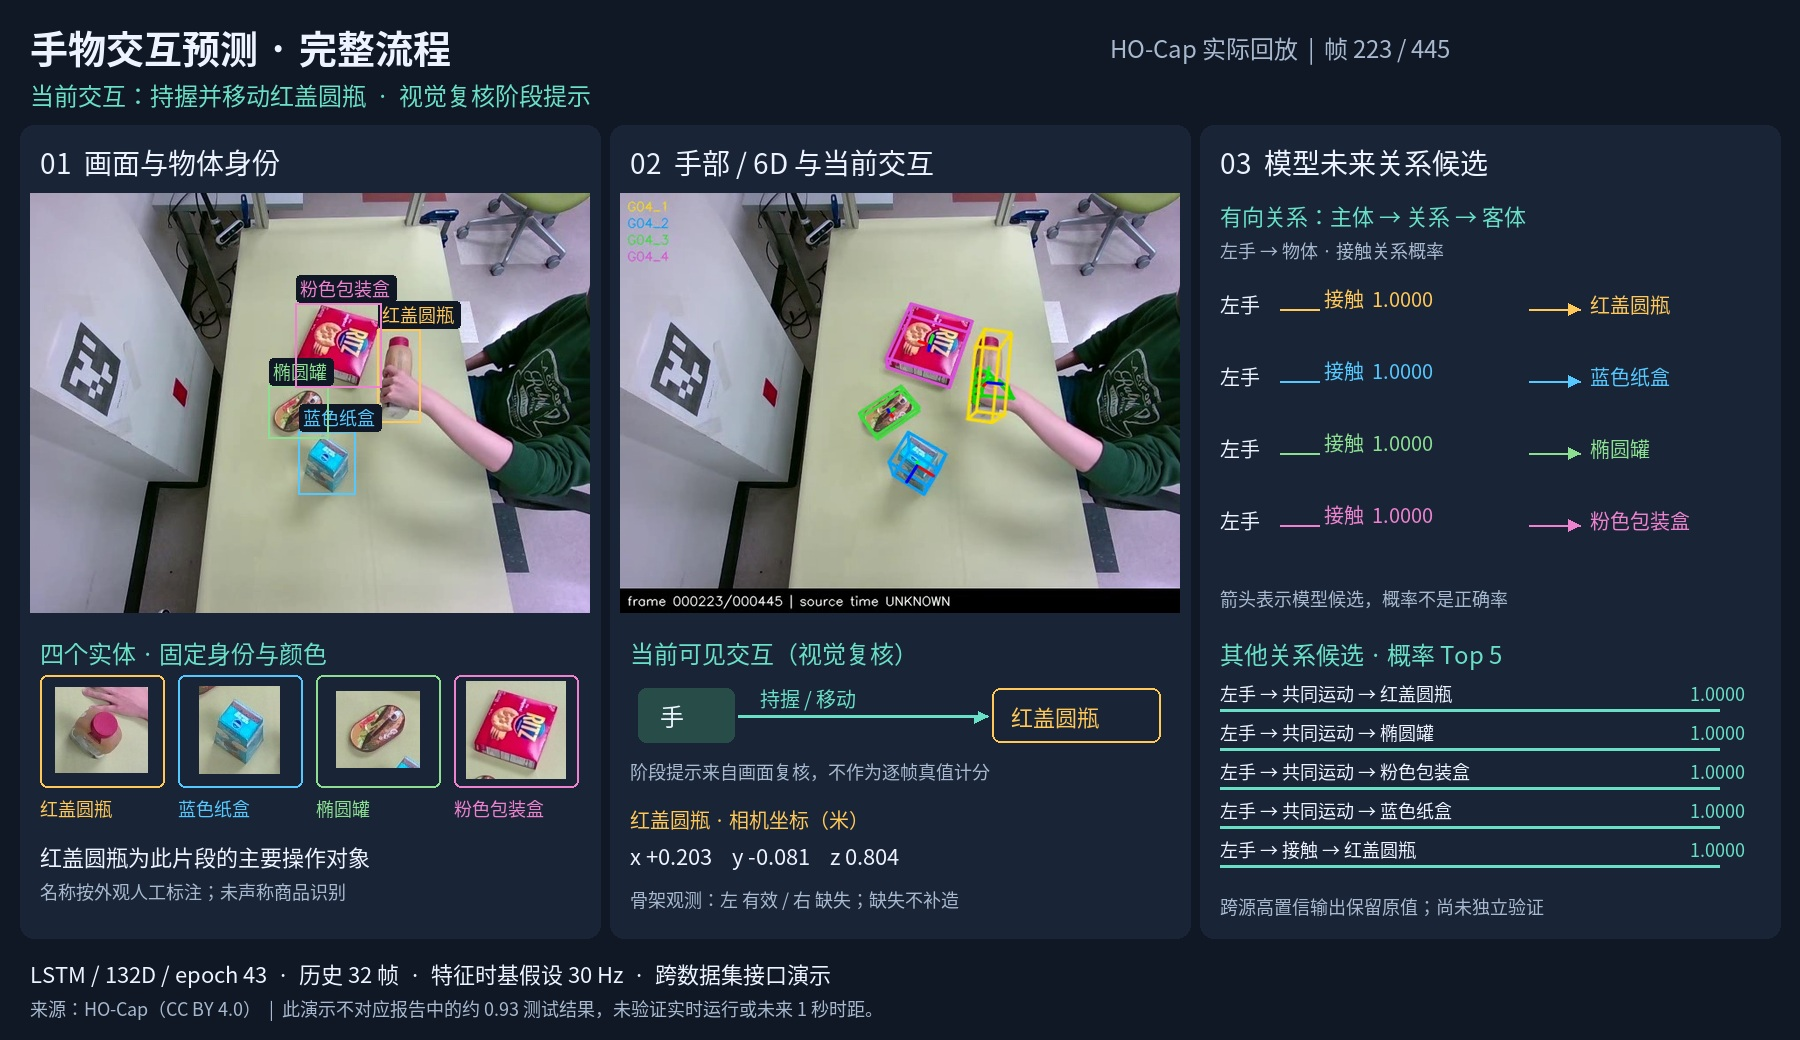
\includegraphics[width=\linewidth]{../04_图片与图表/full_pipeline_demo.jpg}
\caption{新增完整流程的真实演示帧。原始RGB、手部与四物体6D、关系预测并列显示；物体名称与颜色贯穿画面、缩略图与关系客体。中栏显示“手—持握／移动／松手—红盖圆瓶”的视觉复核阶段提示，过渡边界明确标为待核验，不作为逐帧真值。右栏显示左手到各物体的接触候选与概率，下方为全部66种类型中手到物体概率最高的五项。本图是HO-Cap跨数据集接口演示，不属于约0.93结果的测试集。}
\label{fig:demo}
\end{figure}

\textbf{直接播放：}\url{https://egodata-full-pipeline-demo.miracle-techlink.chatgpt.site}。页面提供完整流程、真人手物联合与四物体6D三段实际视频，可慢放、跳转关键帧并下载MP4；PDF中保留关键帧，连续动态内容由播放页呈现。

\subsection{输入、模型与评价边界}
此演示使用\code{lstm\_final}已保存的第43轮checkpoint，输入132维、历史32帧，展示阈值为0.50；没有训练或调参。物体框由已估计6D位姿投影mesh包围盒得到，颜色统计取同帧RGB；物体位姿使用相机坐标。手部仅有二维骨架，未将深度表面点当作度量关节三维，相关特征保持缺失掩码。完整checkpoint哈希和输入说明见播放页的演示清单。跨源输入下可见多条接触和共同运动关系的概率接近1；展示保留原始输出，高置信度不代表正确，不能用画面直接证明泛化。

\textbf{该片段无交互真值，源时戳仍未核验。}演示回放及速度特征采用明确的30Hz假设，不宣称验证了未来1秒预测、实时速度或此片段的F1。它用于检查各模块的贯通与真实输出，不能替代原EgoDemo实验，也不把\code{lstm\_final}文件名等同于最终RSI冠军。阶段测试与项目方最终全量约0.93的结果仍按前文来源分别报告。

\begin{figure}[H]
\centering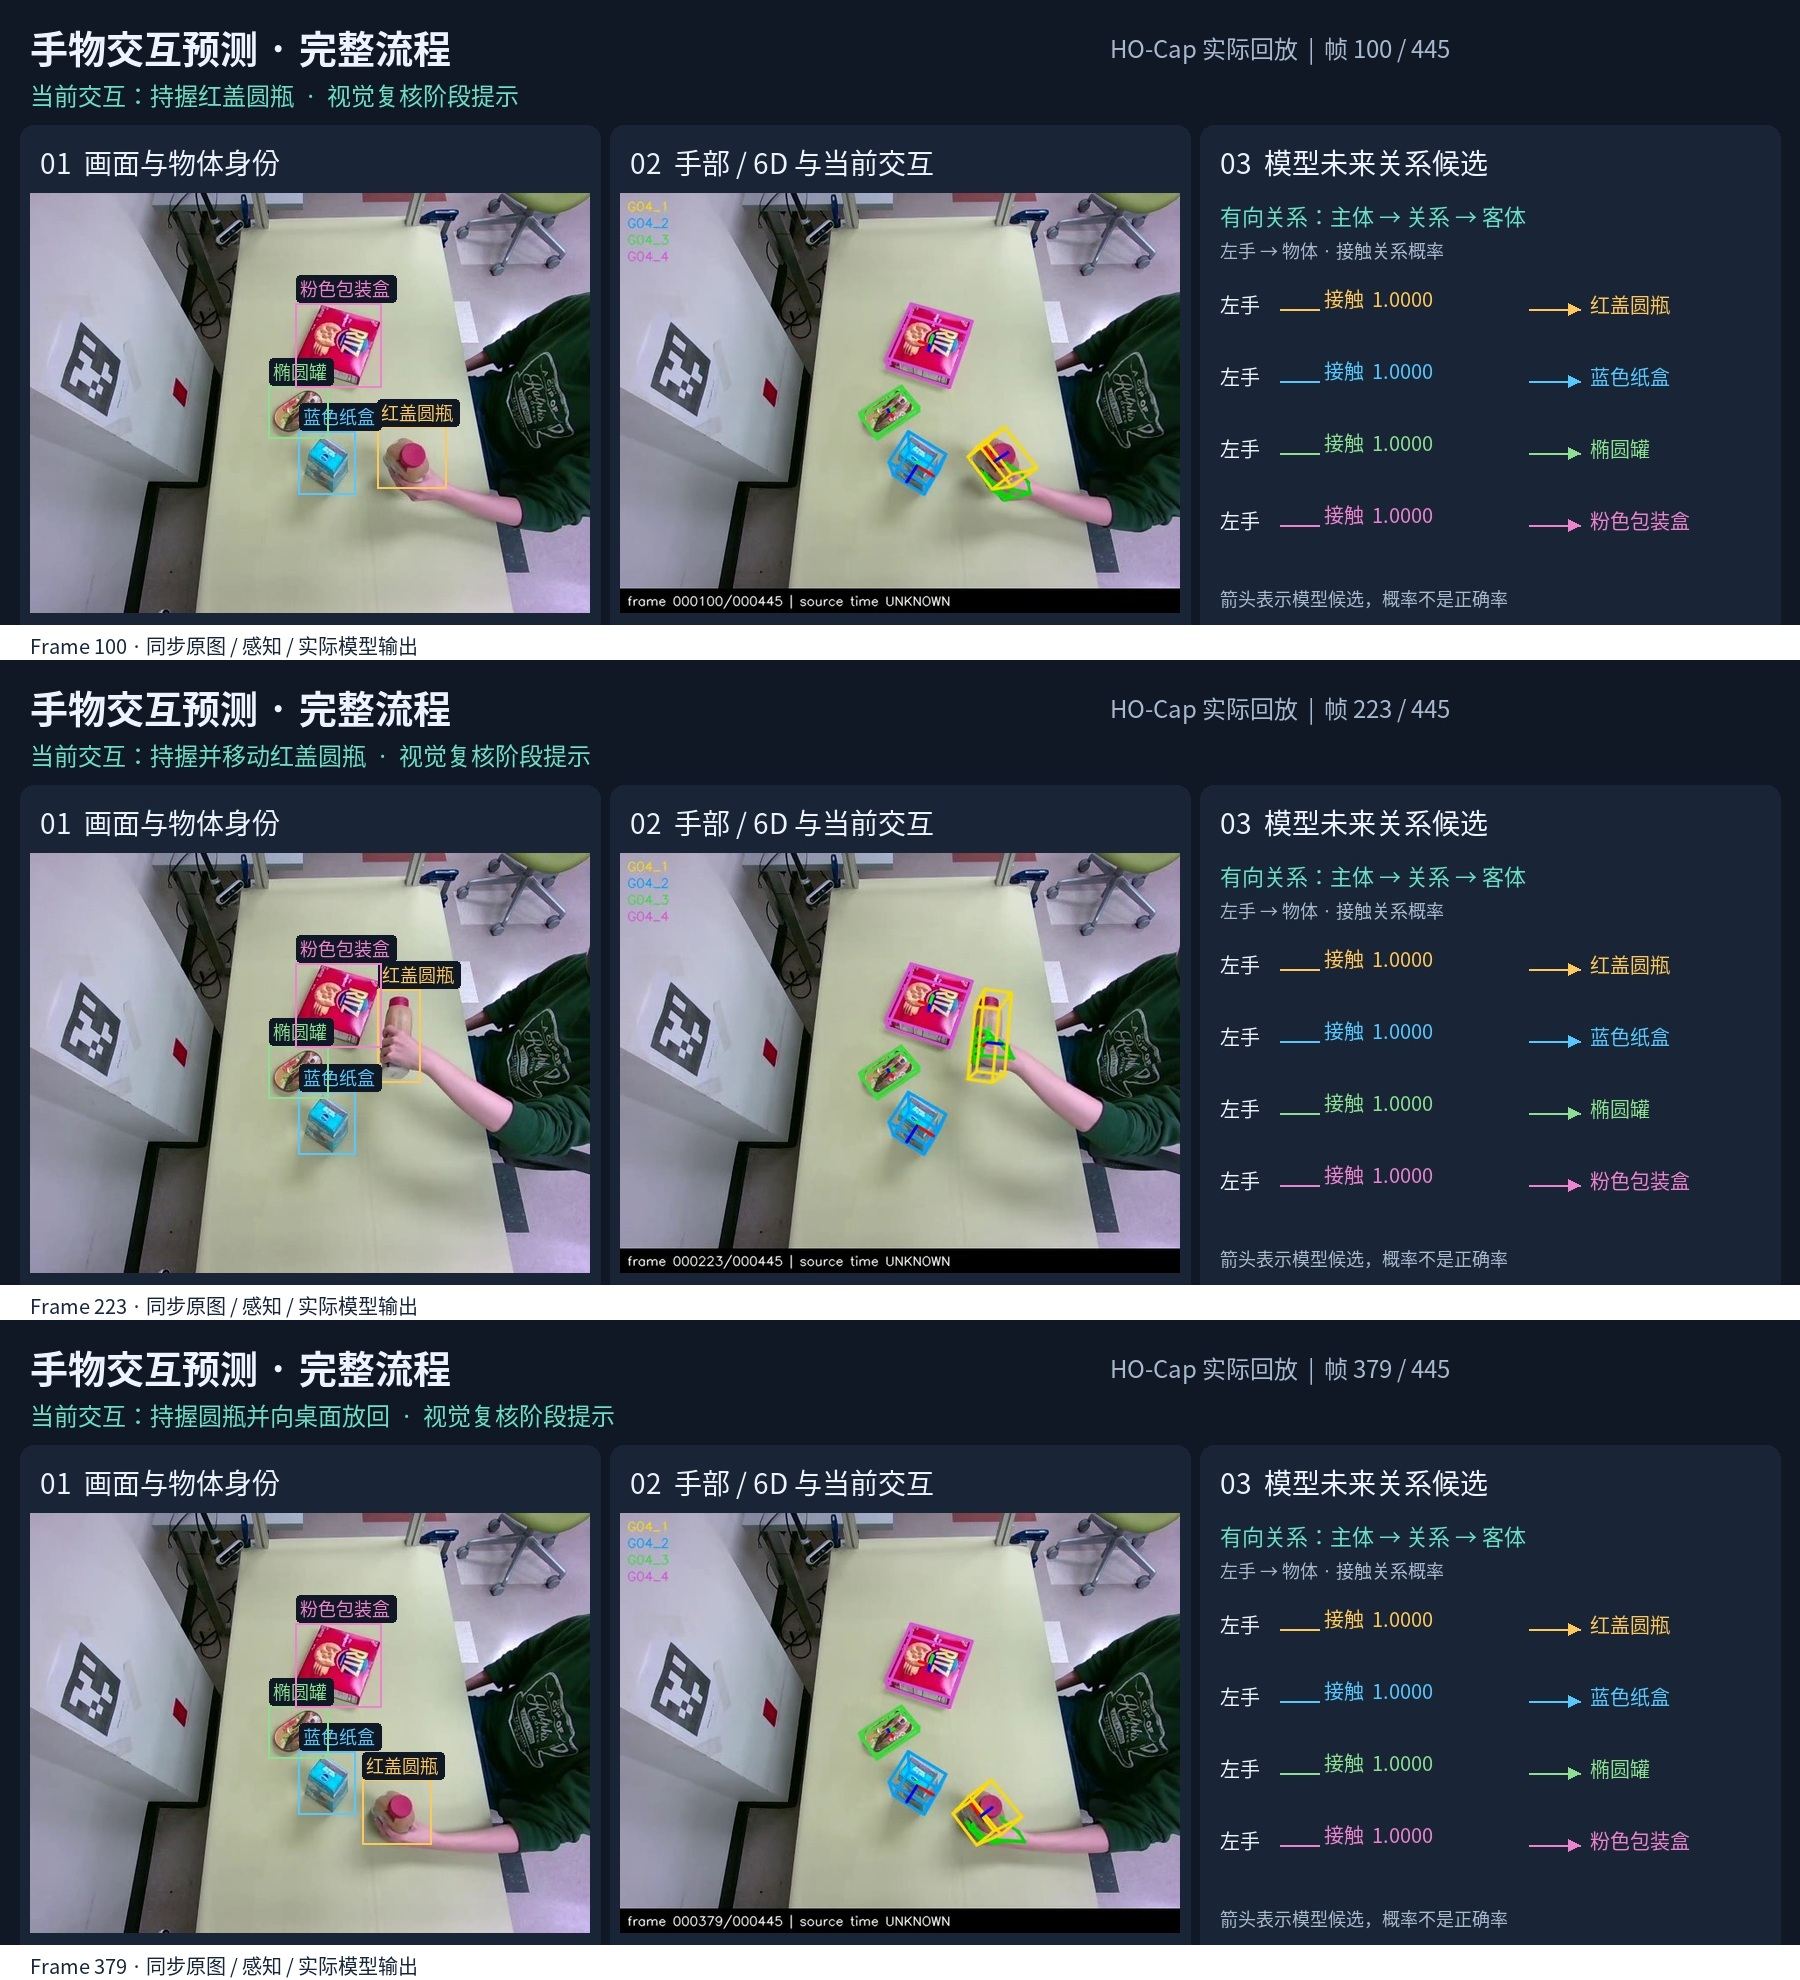
\includegraphics[width=.94\linewidth,height=.65\textheight,keepaspectratio]{../04_图片与图表/full_pipeline_sequence.jpg}
\caption{同一连续演示的第100、223、379帧。三栏分别对应原始画面、感知叠加与实际模型输出；可在播放页跳转到这些帧附近，检查物体移动、骨架与关系输出随时间的变化。该序列没有复核真值，画面不标注预测正确率。}
\label{fig:demo_sequence}
\end{figure}

\subsection{配套演示与离线素材}
精选资料包提供四段视频：HO-Cap完整流程、同源原始RGB、同源四物体感知，以及DexYCB真人手物联合感知。前三段各446帧，DexYCB片段44帧；均保留完整片段与真实输出。打开包内“00\_素材导航.html”即可离线播放。当前物体关系阶段提示来自视觉复核，实际模型概率另列；未对模型失败帧进行筛除。

\section{复现与分析要求}
最终报告需统一四项版本绑定：数据索引与准入文件、特征版本、模型配置／checkpoint、评估器和指标口径。最终全量数据规模应从绑定索引统计，不将资源池、参与处理的采集数和产生有效监督的采集数混为同一数量。

132维增强的上游物体几何包含离线候选，因此在对外说明时应区分条件化预测与严格在线预测。若需要论证全自动实时使用，应单独评价感知误差、身份切换、别名匹配失败及端到端延迟；现有三栏回放不等于实时传感器系统。该边界不改变已完成的交互预测实验，而是明确其使用条件。

对于优化归因，应保留同版本初始配置、冠军配置和每次晋升的验证分数，再独立报告测试结果。最终轮数、成功候选数和数据扩充效果不能根据默认参数或目录名称推断。已有失败候选也应保留，避免搜索账本只剩最终成功项。

\Needspace{10\baselineskip}
\section{结论}
本项目已形成从第一视角数据、视觉复核、手物特征到有向交互图预测的完整技术链。本文补齐了手部与6D位姿原理、真实感知演示及可复算指标图，并在数据扩充、132维位姿增强与多系列RSI中持续优化。项目方报告最终全量结果约0.93；已恢复的扩展阶段原始评估记录显示test micro-F1达到0.939。系统提供了包含物体内容、当前交互与实际预测的连续Demo。本次还直接回收了三个RSI系列的实际账本和阶段评估，并新增带实际模型输出的HO-Cap连续流程演示与视频播放页。后续定稿重点是将指定最终冠军的独立测试与其数据索引绑定，并用同一模型生成正式展示素材。

\FloatBarrier\medskip
\phantomsection\addcontentsline{toc}{section}{参考文献}
{\small\bibliographystyle{ieeenat_fullname}\bibliography{references}}
\clearpage\appendix
\section{公开入口与数据状态}
\begin{itemize}
\item 代码仓库：\url{https://github.com/miracle-techlink/egodata_process}。
\item 报告发布页：\url{https://github.com/miracle-techlink/egodata_process/releases/tag/technical-report-2026-11-12}。
\item ModelScope数据集：\url{https://www.modelscope.cn/datasets/Liuyue9698/ego_pose_dataset}。2026年11月12日直接读取master文件树，只发现README与Git属性文件，尚无数据文件；该地址当前是预留入口。
\item EgoDemo上游入口：\url{https://huggingface.co/datasets/LightwheelAI/EgoDemo}。受限原始材料由上游授权渠道提供。
\end{itemize}

\section{图像来源、署名与公开版范围}
本报告为2026年11月13日素材筛选版。点云和数值验证改用当前HO-Cap真人场景，移除了历史版本对比图与机械臂后端样例；原始阶段指标保持不变。手部坐标与表面运动的公开版替代图为独立绘制的原理示意。新增交互界面与连续关键帧来自真实HO-Cap观测和LSTM推理，属于跨数据集流程演示，并非原EgoDemo测试视频。聚合结果保持相应数据版本，未重新训练或改变模型成绩。

\textbf{DexYCB演示图：}来源为DexYCB，作者Yu-Wei Chao、Wei Yang、Yu Xiang、Pavlo Molchanov、Ankur Handa、Jonathan Tremblay、Yashraj S. Narang、Karl Van Wyk、Umar Iqbal、Stan Birchfield、Jan Kautz和Dieter Fox。数据采用CC BY-NC 4.0，\url{https://dex-ycb.github.io/}；许可\url{https://creativecommons.org/licenses/by-nc/4.0/}。本报告作非商业研究展示，添加了项目估计的手部骨架、物体框与姿态轴，原数据权利保留。

\textbf{HO-Cap演示图：}来源为HO-Cap，作者Jikai Wang、Qifan Zhang、Yu-Wei Chao、Bowen Wen、Xiaohu Guo和Yu Xiang。数据采用CC BY 4.0，\url{https://irvlutd.github.io/HOCap/}；许可\url{https://creativecommons.org/licenses/by/4.0/}。本报告选取已有推理渲染帧并添加物体估计叠加，不暗示作者背书，不分发MANO基础模型。

\section{复现和仍需补充的验证}
报告公式、结构图和聚合统计提供方法与实验口径；真实数据按各上游来源获取。原始索引、逐窗口输出、训练配置和checkpoint在对应授权工作区绑定，不随公开报告再托管。GitHub主分支表示当前已公开实现，不能将工作区全部后续实验能力自动归入某个历史代码提交。

感知仍需对应独立参考的手部误差、物体平移／旋转误差及身份切换统计；覆盖、矩阵自洽和时延分别报告。项目方最终约0.93、扩展阶段可核验的0.938853与后续RSI验证成绩仍按原有范围区分，指定最终运行的独立测试绑定尚需明确。
\end{document}
